\section{Domain Decomposition Methods for Incompressible Flow Simulations}

%cite: Merriam Webster Dictionary http://www.m-w.com/dictionary/decomposition
According to Merriam Webster Dictionary, the term "decomposition" means to separate into constituent parts or elements or into simpler compounds; one of the definition for "domain" is a region distinctively marked by some physical feature.

Mathematically, "decomposition" means a rewriting of a given quantity in terms of a combination of simpler quantities; "domain" means the set for which a function is defined, a connected open set in topology, or a commutative ring that has an identity element but zero divisors \cite{Weisstein}.

%cite: Eric W. Weisstein. "Domain." From MathWorld--A Wolfram Web Resource. Eric W. Weisstein. "Decomposition." From MathWorld--A Wolfram Web Resource.  %http://mathworld.wolfram.com/Domain.html %http://mathworld.wolfram.com/Decomposition.html

Here domain decomposition methods are referred to the techniques for dividing numerical problems into smaller parts, solving each piece, and then, if wished, merging them back to assemble the whole solution. Comprehensive reviews of the domain decomposition method for partial differential equations can be found in the references \cite{Toselli05, Quarteroni1999}.

\normalsize
\subsection*{Schwarz Method}
\begin{figure}[htbp]
  \begin{center}
    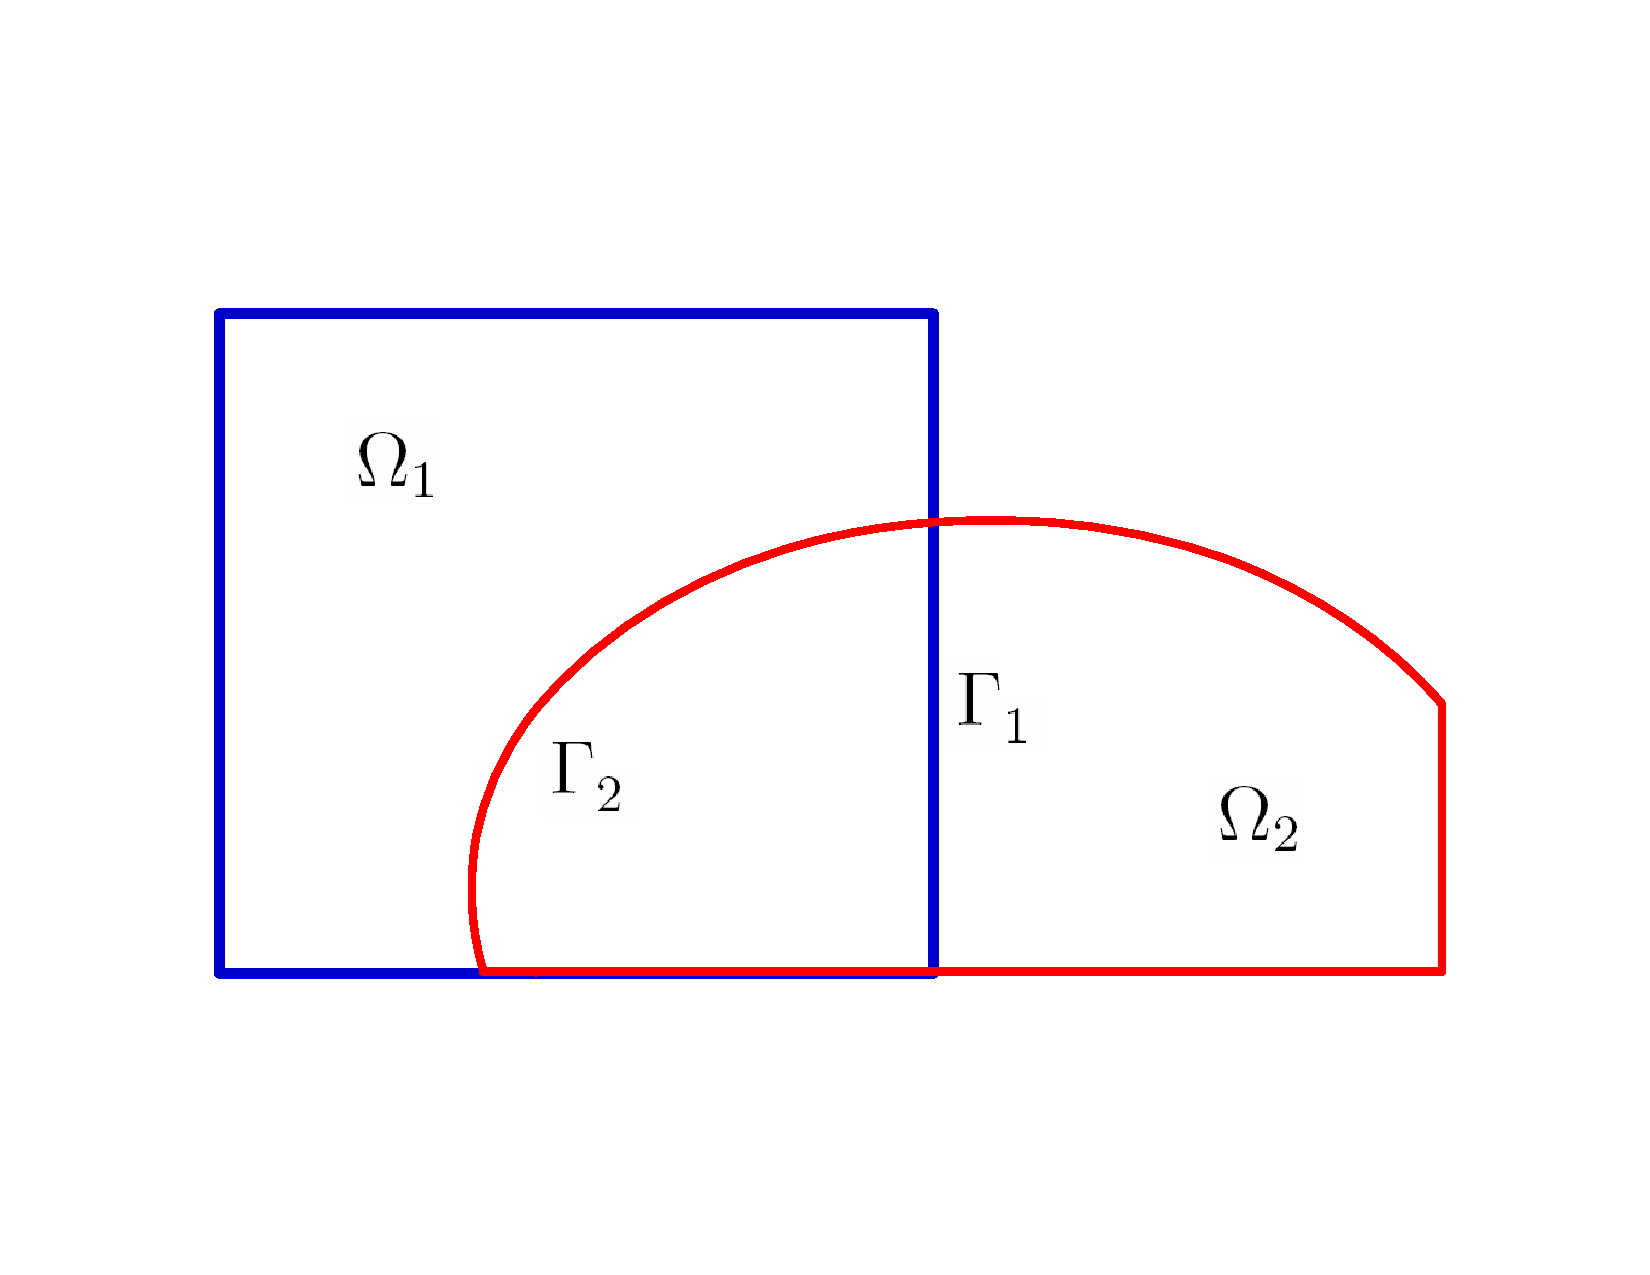
\includegraphics[scale=0.3]{../figures/Schwarz.pdf}
    \caption{Overlapping Schwarz Method.}
    \label{fig:Schwarz}
  \end{center}
\end{figure}
The Schwarz alternating method \cite{Schwarz1869} can be used to decompose the solution domain of iterative solvers for the Poisson equation. For a simplified two-subdomain case, the partial differential equation is first solved in subdomain $\Omega_1$ with Dirichlet boundary condition on the boundary $\Gamma_1$,
\be
\left\{
\baa{ccccc}
A_{1}\phi_1^n & = & B_1   & in & \Omega_1 \\
\phi_1^n    & = & \phi_2^{n-1}|_{\Gamma_1} & on & \Gamma_1
\eaa
\right.
\label{eqn:Schwarz-multi-1}
\ee %u_1^n    & = & g     & in & \p \Omega_1 \backslash \Gamma_1\\
and then the value on the subdomain boundary $\Gamma_2$ is copied from the overlapping nodes inside $\Omega_1$, continuing the solving process in subdomain $\Omega_2$,
\be
\left\{
\baa{ccccc}
A_{2}\phi_2^{n+1} & = & B_2                   & in & \Omega_2 \\
\phi_2^{n+1}    & = & \phi_1^{n}|_{\Gamma_2} & on & \Gamma_2
\eaa
\right.
\label{eqn:Schwarz-multi-2}
\ee %u_2^n    & = & g         & in & \p \Omega_2 \backslash \Gamma_2 \\

An altered version replaces the boundary value $\phi_1^{n}|_{\Gamma_2}$ in Equation \ref{eqn:Schwarz-multi-2} with the previous value $\phi_1^{n-1}|_{\Gamma_2}$, enabling the simultaneous solving of the two subdomains.
\be
\left\{
\baa{ccccc}
A_{2}\phi_2^n & = & B_2                   & in & \Omega_2 \\
\phi_2^n    & = & \phi_1^{n-1}|_{\Gamma_2} & on & \Gamma_2
\eaa
\right.
\ee %u_2^n    & = & g         & in & \p \Omega_2 \backslash \Gamma_2 \\
The boundary conditions for subdomains can be further generalized to Robin type, allowing the non-overlapping between subdomains.
\be
\left\{
\baa{ccccc}
A_{1}\phi_1^n & = & B_1       & in & \Omega_1 \\
\alpha_{1}\f{\p \phi_1^n}{\p \eta_{12}}+ \lambda_{1}\phi_1^{n}    & = & -\alpha_{1}\f{\p \phi_2^{n-1}}{\p \eta_{21}}+ \lambda_{1}\phi_1^{n-1} & in & \p \Omega_1 \cap \p \Omega_2
\eaa
\right.
\ee %\phi_1^n    & = & g         & in & \p \Omega_1 \cap \p \Omega \\
\be
\left\{
\baa{ccccc}
A_{2}\phi_2^n & = & B_2       & in & \Omega_2 \\
\alpha_{2}\f{\p \phi_2^n}{\p \eta_{21}}+ \lambda_{2}\phi_2^{n}    & = & -\alpha_{2}\f{\p \phi_1^{n}}{\p \eta_{12}}+ \lambda_{2}\phi_1^{n} & in & \p \Omega_2 \cap \p \Omega_1
\eaa
\right.
\ee %\phi_2^n    & = & g         & in & \p \Omega_2 \cap \p \Omega \\

An example of incompressible flow simulations using Schwarz alternating method with the spectral element formulation is demonstrated by Fischer \cite{Fischer1997}.

\normalsize
\subsection*{Substructuring Method}
\begin{figure}[htbp]
  \begin{center}
    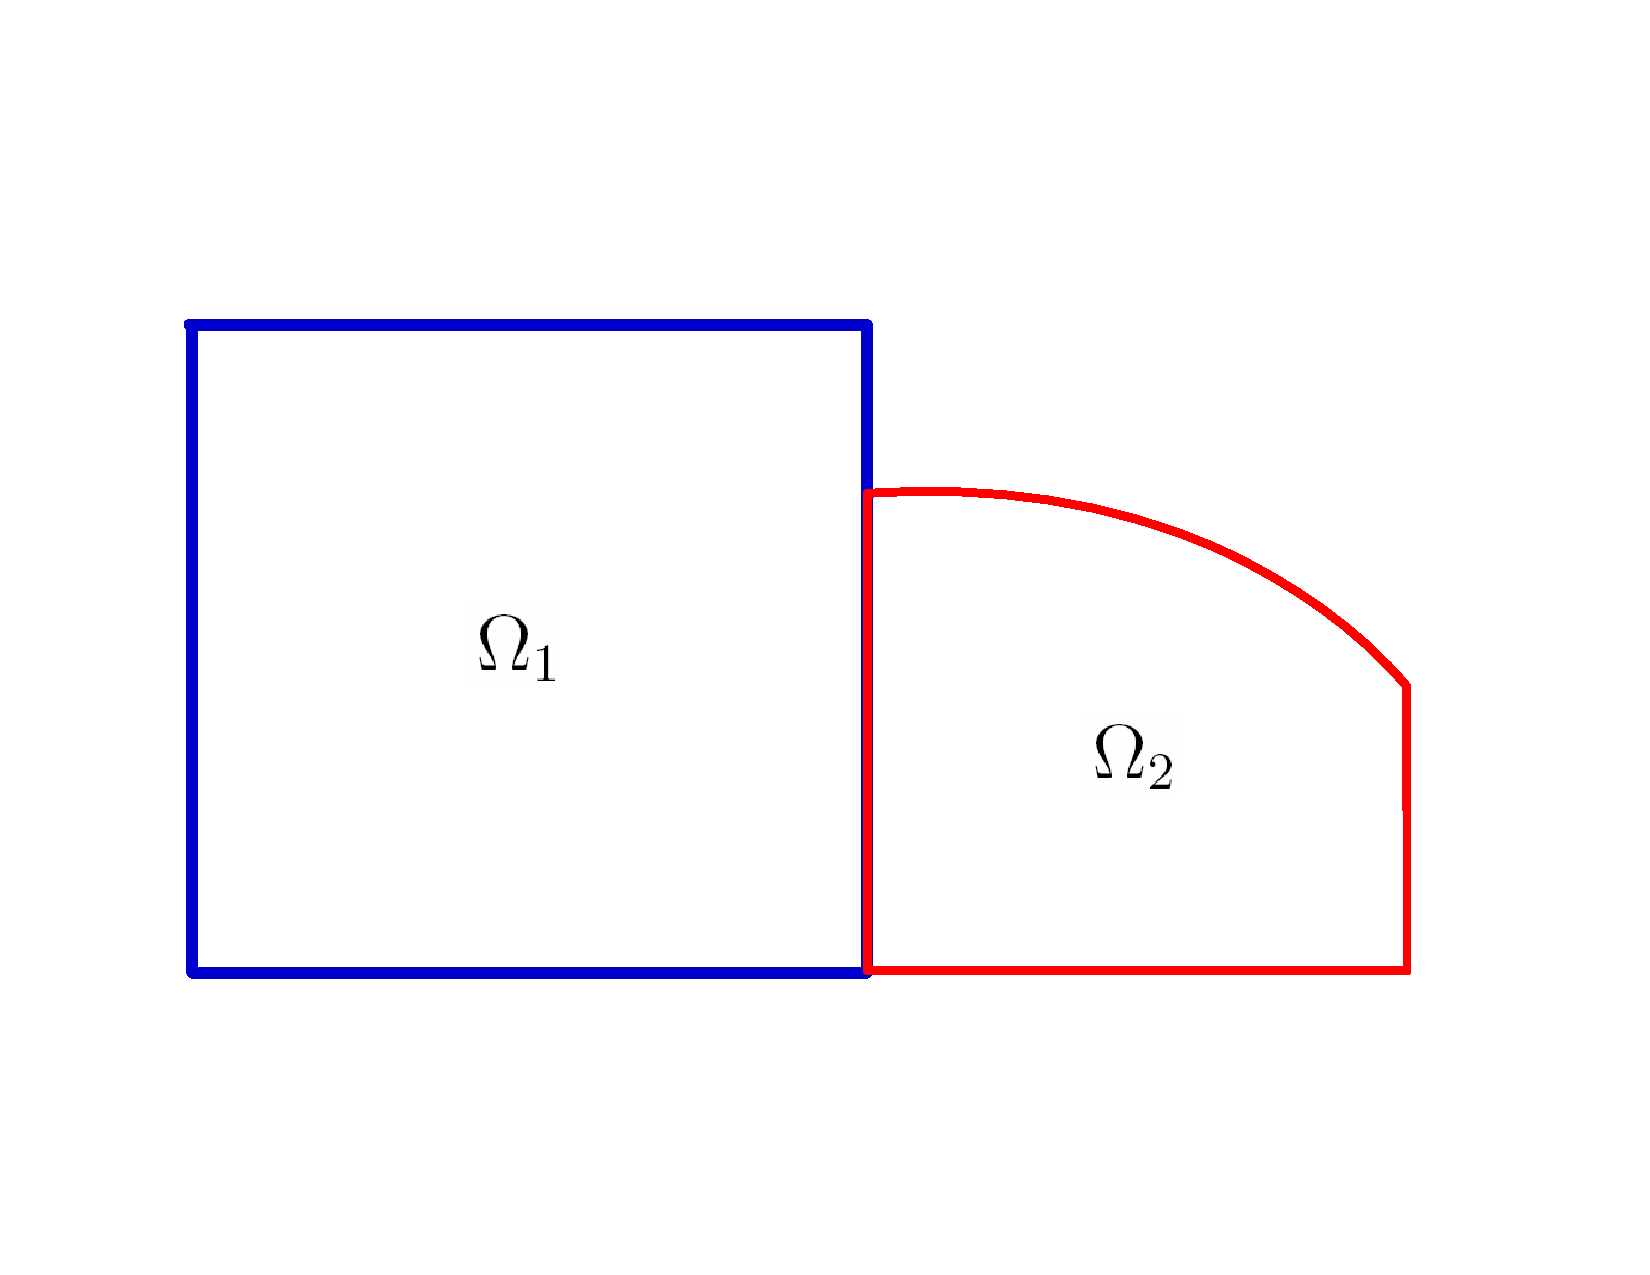
\includegraphics[scale=0.3]{../figures/Nonoverlapping.pdf}
    \caption{Non-Overlapping Method.}
    \label{fig:Nonoverlapping}
  \end{center}
\end{figure}

The linear system obtained from the discretization of the incompressible Navier-Stokes equation can be rearranged such that the unknowns on the interfaces of subdomains can be solved independently from the rest unknowns.

Consider a domain $\Omega$ which is divided into two subdomains $\Omega_1$, $\Omega_2$, and interface $\Gamma$. The system of the discretized partial differential equations for the whole domain $\Omega$ can be written in the matrix form:
\be
\left[
\begin{array}{ccc}
A_{11} & 0 & A_{1\Gamma}\\
0 & A_{22} & A_{2\Gamma}\\
A_{\Gamma 1} & A_{\Gamma 2}  & A_{\Gamma \Gamma}\\
\end{array}
\right]
\left[
\begin{array}{c}
\phi_{1}\\
\phi_{2}\\
\phi_{\Gamma}\\
\end{array}
\right]
=
\left[
\begin{array}{c}
B_{1}\\
B_{2}\\
B_{\Gamma}\\
\end{array}
\right]
\ee
where $\phi_1$ and $\phi_2$ are the variables inside the subdomains, $\phi_{\Gamma}$ contains the variables on the interface $\Gamma$. The system for the variables on the interface can be derived as:
\be
S \ \phi_{\Gamma }=b_{\Gamma}-A_{\Gamma i}A_{i}^{-1}B_i
\label{eqn:Schur-interface}
\ee
where $S$ is the Schur complement of the submatrix $A_{i}$,
\be
S=A_{\Gamma \Gamma}-A_{\Gamma i}A_{i}^{-1}A_{i \Gamma}
\ee
and $A_i$, $A_{\Gamma i}$, $A_{i \Gamma}$, $B_i$ are defined as:
\be
A_i=
\left[
\begin{array}{cc}
A_{11} & 0 \\
0 & A_{22}
\end{array}
\right]
\ee
\be
A_{\Gamma i}=(A_{\Gamma 1},A_{\Gamma 2}), \ \
A_{i \Gamma}=(A_{1 \Gamma},A_{2 \Gamma})^T , \ \
B_i=(B_1,B_2)^T
\ee
After the solution on the interface in Equation \ref{eqn:Schur-interface} is found, the two subdomains can be independently solved with the Dirichlet boundary condition on the interface. Couzy \cite{Couzy1995} demonstrated this technique with the spectral element formulation for incompressible flow simulations.

%\input{Chapter5-DDM-Incompressible-Explicit-SRM}

